\scanpage{18}

\textbf{ACADEMIE D'AIX-MARSEILLE}\\
\rule{3cm}{.4pt}\\
\textbf{INSPECTION ACADEMIQUE}\\
\textbf{DE VAUCLUSE}\\
\rule{1cm}{.4pt}

\figure{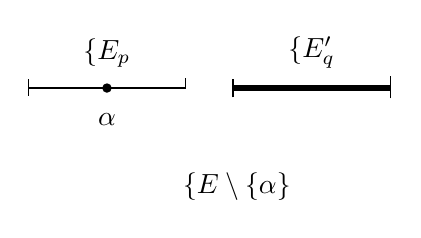
\begin{tikzpicture}[x=1cm,y=1cm]
\draw (0,0)--(2,0);\draw (0,-.10)--(0,.12);\draw (2,0)--(2,.13);\fill (1,0) circle (.06);
\node at (1,.45) {$\{E_p$};\node at (1,-.40) {$\alpha$};
\draw[line width=2pt] (2.6,0)--(4.6,0);\draw (2.6,-.12)--(2.6,.12);\draw (4.6,-.13)--(4.6,.15);
\node at (3.6,.45) {$\{E'_q$};
\node at (2.65,-1.25) {$\{E\setminus\{\alpha\}$};
\end{tikzpicture}}
\margin{$p\geq$}
\margin{278}

% Global cancellation is the manuscript's X, not a linewise sout.
\begingroup
\newsavebox{\SPXCIIICancelledXVIII}
\begin{lrbox}{\SPXCIIICancelledXVIII}
\begin{minipage}{\linewidth}

\[
\begin{gathered}
F=\varinjlim_{A/F}\alpha\\
G=\varinjlim_{A/G}\beta
\end{gathered}
\]

\[
\begin{aligned}
F\times G&=\varinjlim_{A/F}\text{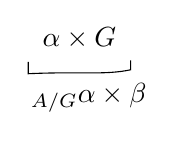
\begin{tikzpicture}[baseline=(e.base)]\node[inner sep=0pt] (e) at (0,0) {$\alpha\times G$};\draw (-0.65,-.3)--(-0.65,-.45)..controls(0,-.42)and(0.325,-.47)..(0.65,-.4)--(0.65,-.28);\node[anchor=north,inner sep=0pt] at (.12,-.57) {$\displaystyle \varinjlim_{A/G}\alpha\times\beta$};\end{tikzpicture}}\\
&=\varinjlim_{A/F\times A/G}\alpha\times\beta
\end{aligned}
\]

\par\noindent
\makebox[0pt][r]{%
  \smash{\begin{tabular}[t]{@{}l@{}}
  $\alpha\unsure{-|\longrightarrow}F$\\$\beta\unsure{-|\longrightarrow}G$
  \end{tabular}}\hspace{.75em}%
}\par

\figure{\begin{tikzpicture}[x=1cm,y=1cm]
\node[anchor=west] (prod) at (2.2,0) {$\displaystyle
\varphi_!(F\times G)=\varinjlim_{A/F\times A/G}
\text{\begin{tikzpicture}[baseline=(e.base)]\node[inner sep=0pt] (e) at (0,0) {$\varphi_!(\alpha\times\beta)$};\draw (-1.0,-.3)--(-1.0,-.45)..controls(0,-.42)and(0.5,-.47)..(1.0,-.4)--(1.0,-.28);\node[anchor=north,inner sep=0pt] at (.12,-.57) {$\displaystyle \varphi_!(\alpha)\times\varphi_!(\beta)$};\end{tikzpicture}}$};
\node[anchor=west] at (1,-1.55) {$\displaystyle\varphi_!(F)=\varinjlim_{A/F}\varphi_!(\alpha)$};
\node[anchor=west] at (1,-2.55) {$\displaystyle\varphi_!(G)=\varinjlim_{A/G}\varphi_!(\beta)$};
\draw ([xshift=-.25cm,yshift=.25cm]prod.north east)
 .. controls ++(.55,.25) and ++(.45,0) .. ([xshift=.35cm]prod.north east)
 -- ([xshift=.35cm,yshift=-.15cm]prod.south east)
 .. controls ++(0,-.25) and ++(.65,-.05) .. (8,-.95)
 .. controls (8.05,-1.65) and (8.7,-2.85) .. (7.4,-3.05)
 -- (1.4,-3.3)
 .. controls (.7,-3.4) and (.5,-3.1) .. (.5,-2.7)
 -- (.5,-.8) -- (-.4,-.95);
\end{tikzpicture}}

\diagram{\begin{tikzcd}[ampersand replacement=\&,column sep=small]
A\&{\unsure{\overset{\varphi}{\rule{1cm}{.4pt}}|\xrightarrow{\varphi}}}\&\mathcal X
\end{tikzcd}}

\diagram{\begin{tikzcd}[ampersand replacement=\&]
C=\mathcal X\arrow[r,shift right=2,"{\unsure{u|v}=\varphi^*}"']\&C'=\widehat A\arrow[l,shift right=2,"{\unsure{v|u}=\varphi_!}"']
\end{tikzcd}}

\figure{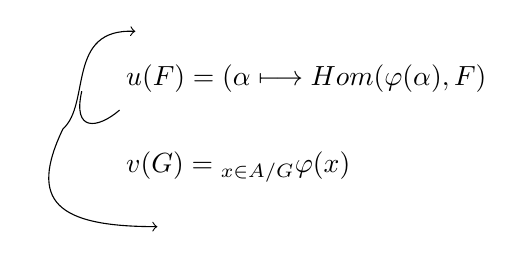
\begin{tikzpicture}[x=.8cm,y=.8cm]
\node[anchor=west] at (1.05,2.05) {$u(F)=(\alpha\longmapsto\operatorname{Hom}(\varphi(\alpha),F)$};
\node[anchor=west] at (1.05,.65) {$v(G)=\displaystyle\varinjlim_{x\in A/G}\varphi(x)$};
\draw[<->] (1.35,2.8) .. controls (.25,2.85) and (.65,1.65) .. (.2,1.25)
 .. controls (-.35,.1) and (.1,-.3) .. (1.7,-.3);
\draw (.5,1.85) .. controls (.35,1.2) and (.75,1.25) .. (1.1,1.55);
\end{tikzpicture}}

\par\noindent
\makebox[\linewidth][r]{%
  \smash{\begin{tabular}[t]{@{}l@{}}
  $u$ continu\\$v$ cocontinu
  \end{tabular}}%
}\par

\diagram{\begin{tikzcd}[ampersand replacement=\&,row sep=small,column sep=large]
\mathcal X\arrow[r]\&\widehat A\&\&\\
Y\&/\;a_i\to\varphi^*(Y)\&\varphi(a_i)\arrow[r]\&Y
\end{tikzcd}}

\end{minipage}
\end{lrbox}
\begin{center}
\begin{tikzpicture}
\node[anchor=south west,inner sep=0pt,outer sep=0pt] (spCancelledXVIII) at (0,0)
  {\usebox{\SPXCIIICancelledXVIII}};
% The unit vectors are the saved block's width and height.
\begin{scope}[x={(spCancelledXVIII.south east)},y={(spCancelledXVIII.north west)}]
% Descending course: upper left to lower right.
\draw[line width=.45pt] (.09,1.035)
 .. controls (.14,.96) and (.17,.84) .. (.26,.70)
 .. controls (.42,.49) and (.68,.15) .. (.81,.01);
% Opposing course, with the source's short upper pen gap.
\draw[line width=.45pt] (.50,1.00)
 .. controls (.50,.96) and (.44,.87) .. (.42,.835);
\draw[line width=.45pt] (.41,.812)
 .. controls (.36,.65) and (.21,.28) .. (.15,.13)
 .. controls (.145,.10) and (.14,.09) .. (.13,.08);
\end{scope}
\end{tikzpicture}
\end{center}
\endgroup

\margin{17}
